\chapter[Clustered calibration plots]{Clustered flexible calibration plots for binary outcomes using random effects modeling}
% Only include if the thesis is written as a collection of papers
%_________________________
\label{sec:chp_ClusteredCalibration}

\glsunset{ADNEX}
\glsunset{AUC}
\glsunset{CGC}
\glsunset{CI}
\glsunset{CPM}
\glsunset{DGM}
\glsunset{EPC}
\glsunset{GLMM}
\glsunset{ICC}
\glsunset{IOTA}
\glsunset{IPD}
\glsunset{MIXC}
\glsunset{MSCE}
\glsunset{OSF}
\glsunset{PI}
\glsunset{TMAC}
\glsunset{TRIPOD}


published as:
\begin{quote}
Barre\~{n}ada L, De Cock Campo B, Wynants L \& Van Calster B. Clustered flexible calibration plots for binary outcomes using random effects modeling. Research Synthesis Methods. 2025;1--22. https://doi.org/10.1017/rsm.2025.10046
\end{quote}
%_________________________

\section*{Abstract}
Evaluation of clinical prediction models across multiple clusters, whether centers or datasets, is becoming increasingly common. A comprehensive evaluation includes an assessment of the agreement between the estimated risks and the observed outcomes, also known as calibration. Calibration is of utmost importance for clinical decision making with prediction models and it may vary between clusters. We present three approaches to take clustering into account when evaluating calibration. (1) Clustered group calibration (\gls{CGC}), (2) two-stage meta-analysis calibration (\gls{TMAC}) and (3) mixed model calibration (\gls{MIXC}) can obtain flexible calibration plots with random effects modelling and providing confidence and prediction intervals. As a case example, we externally validate a model to estimate the risk that an ovarian tumor is malignant in multiple centers (N = 2489). We also conduct a simulation study and synthetic data study generated from a true clustered dataset to evaluate the methods. In the simulation study \gls{MIXC} and \gls{TMAC} (splines) gave estimated curves closest to the true overall curve. In the synthetic data study \gls{MIXC} produced cluster specific curves closest to the truth. Coverage of the prediction interval across the plot was best for \gls{TMAC} with splines. We recommend using \gls{TMAC} with splines to estimate the overall curve and the 95\% \gls{PI} and \gls{MIXC} for the cluster specific curves, especially when sample size per cluster is limited. We provide ready-to-use code to construct summary flexible calibration curves with confidence and prediction intervals to assess heterogeneity in calibration across datasets or centers.

\section{Introduction}
Clinical prediction models (\glspl{CPM}) are evidence-based tools that estimate the probability of health-related events either at the time of evaluation (diagnosis) or at some point in the future (prognosis) \cite{steyerbergClinicalPredictionModels2019a,vansmedenClinicalPredictionModels2021}. These risk estimates play a crucial role in evidence-based decision-making and can be of great value when counselling patients. However, to ensure the reliability of risk estimates, \glspl{CPM} must exhibit good calibration \cite{vancalsterCalibrationHierarchyRisk2016}. Calibration assesses how well the predicted risks correspond to observed risks \cite{vancalsterCalibrationHierarchyRisk2016}. In recent years, there has been a notable increase in studies involving multiple clusters. The term "cluster" can refer to different groupings within the population under study, depending on the context. For example, in multicenter studies, a cluster commonly refers to different centers, whereas in meta-analysis, a cluster may pertain to each study or centers within the study where possible (e.g. individual patient data (\gls{IPD}) meta-analysis \cite{rileyIndividualParticipantData2021a}). In this work, the term "cluster" will specifically denote a center in a multicenter study, but the methods proposed apply more generally as well. An analysis of \glspl{CPM} included in Tufts PACE (Predictive Analytics + Comparative Effectiveness), developed after the year 2000, revealed that 64\% of the models utilized multicenter (clustered) data, indicating a growing trend in such studies \cite{wynantsUntappedPotentialMulticenter2019,wesslerTuftsPACEClinical2017}. \gls{TRIPOD} (Transparent Reporting of a Multivariable Prediction Model for Individual Prognosis or Diagnosis) has addressed this development by publishing an extension known as \gls{TRIPOD}-Cluster \cite{debrayTransparentReportingMultivariable2023}. This extension underscores the importance of taking clustering into account when developing or evaluating prediction models.

Miscalibration can have a harmful influence on medical decision making \cite{vancalsterCalibrationRiskPrediction2015}. It is common to observe heterogeneity in model performance across centers or studies, most notably in model calibration \cite{vancalsterValidationModelsDiagnose2020,guptaDevelopmentValidationISARIC2021,steyerbergAssessmentHeterogeneityIndividual2019,vanAmsterdamCausalViewpoint2024}. It can thus be misleading to generalize performance results from single-cluster data \cite{wynantsDoesIgnoringClustering2018,debrayFrameworkDevelopingImplementing2013,dejongDevelopingMoreGeneralizable2021,moherGuidanceDevelopersHealth2010}. For these reasons, it is crucial to collect clustered data to investigate and quantify heterogeneity in calibration performance between clusters. The presence of clustering introduces challenges, as individuals are no longer independent due to correlations among patients within the same cluster \cite{snijdersMultilevelAnalysisIntroduction2012,finchMultilevelModelingUsing2019a}. Traditional (non-clustered) methodologies should therefore be adapted for use with clustered data.

The most informative assessment of calibration performance for a prediction model is a calibration plot, used to assess whether, among patients with the same estimated risk of the event, the observed proportion of events equals the estimated risk \cite{vancalsterCalibrationHierarchyRisk2016,vancalsterPerformanceEvaluationPredictive2024}.A calibration plot has estimated risks on the x-axis, and the observed proportion on the y-axis. For binary outcomes, observed outcome values are \(Y = 0\) (no event) or \(Y = 1\) (event). The observed proportion of individuals with the event conditional on estimated risk are not observed directly, but are estimated. One approach consists of creating \(Q\) groups (usually based on quantiles of estimated risks) and estimating the observed proportion in each of the groups as the proportion of individuals with the condition. We refer to this approach throughout the text as grouped calibration. The calibration plot then has \(Q\) dots representing the mean risk (value on the x-axis) and observed proportion (value on the y-axis). Another approach is using a flexible model \cite{austinGraphicalAssessmentInternal2014}. The observed outcome is regressed on the estimated probabilities using a smoother such as local regression (loess) or splines. The smoothed relation or \(Q\) groups are plotted together with a line of identity which represents perfect calibration. The grouped approach loses information by categorizing the estimated risks, and depends on the value of \(Q\) and the grouping approach. Flexible models are dependent on smoothing parameters. Flexible calibration curves have been presented for different problems like survival models \cite{austinGraphicalCalibrationCurves2020}, competing risk models \cite{austinGraphicalCalibrationCurves2022}, or multiclass models \cite{vanhoordeSplinebasedToolAssess2015}. Flexible calibration curves that consider clustering have been understudied. Although summarizing statistics of calibration (e.g. O:E) can be meta-analysed across clusters, such summarizing statistics are by definition less informative than the calibration plot \cite{vancalsterPerformanceEvaluationPredictive2024,debrayGuideSystematicReview2017}. We present three different approaches to construct flexible calibration curves from clustered data, provide cluster-specific curves, and quantify heterogeneity using prediction intervals. We illustrate the methodologies with a real case example on ovarian cancer data and compare the performance of the methodology using simulated data, and synthetic data. Section 2 presents the motivating example, the general notation used through the paper, and introduces the three approaches to obtain calibration plots accounting for clustering. Section 3 and 4 present the methodology and results of the simulation study and synthetic data analysis, respectively, and in section 5 we conclude by discussing our findings. This study is an initial assessment of methods for clustered calibration analysis that we classify as a phase 2 methodological study in the four phase framework from Heinze and colleagues \cite{heinzePhasesMethodologicalResearch2024}.

\section{Methods}
\subsection{\texorpdfstring{Motivating example: ADNEX model and Ovarian cancer data}{Motivating example: ADNEX model and Ovarian cancer data}}
The methods will be illustrated using the \gls{ADNEX} model for ovarian tumor discrimination that was developed with data from the International Ovarian Tumor Analysis (\gls{IOTA}) group \cite{vancalsterEvaluatingRiskOvarian2014,timmerman2024}. The \gls{ADNEX} model is a multinomial regression mixed model with random intercepts per center to estimate the probability that an ovarian mass is malignant. Predicting malignancy of ovarian masses prior to surgery is important because benign masses can be managed conservatively, and malignant masses require different surgical approaches depending on the malignant subtype. \gls{ADNEX} estimates the risk of five outcomes: benign tumor, borderline tumor, stage I invasive cancer, stage II-IV invasive cancer, and secondary metastasis. This work will focus on the overall risk of malignancy, which is obtained by adding the risks for the malignant subtypes. \gls{ADNEX} has three clinical and six ultrasound predictors: age, serum CA125 level, type of center (oncology center or other hospital type), maximal diameter of the lesion, proportion of solid tissue, number of papillary projections, presence of \textgreater10 locules, acoustic shadows, and ascites. CA125 is optional, and in this work we focus on \gls{ADNEX} without CA125. \gls{ADNEX} coefficients already capture some of the between-center heterogeneity through the type of center. To illustrate multicenter calibration of the \gls{ADNEX} model we use an external validation dataset of 2489 patients recruited in 17 hospitals \cite{kaijserEvidencebasedApproachDiagnosis2015}. Previous external validation of \gls{ADNEX} on this dataset suggested that there was important heterogeneity between hospitals (Figure S1) \cite{vancalsterValidationModelsDiagnose2020}. To avoid computation errors, three small non-oncology centers in Italy were combined, as well as two small non-oncology centers in the United Kingdom. The dataset then contains 14 clusters, with a median number of 189 patients per cluster (range 38 to 360) (Figure~\ref{fig:4:1}). The mean estimated probabilities (range 0.10 to 0.53) and the prevalence of malignancy (range 0.16 to 0.72) varied between clusters. The intra-cluster correlation (\gls{ICC}) in (logit) malignancy risk based on the null random intercept model is 15\% \cite{snijdersMultilevelAnalysisIntroduction2012}. An \gls{ICC} of 0 would mean that all clusters are similar, and all variance in the logit malignancy risk is due to individual-level variability.

\begin{figure}
\centering
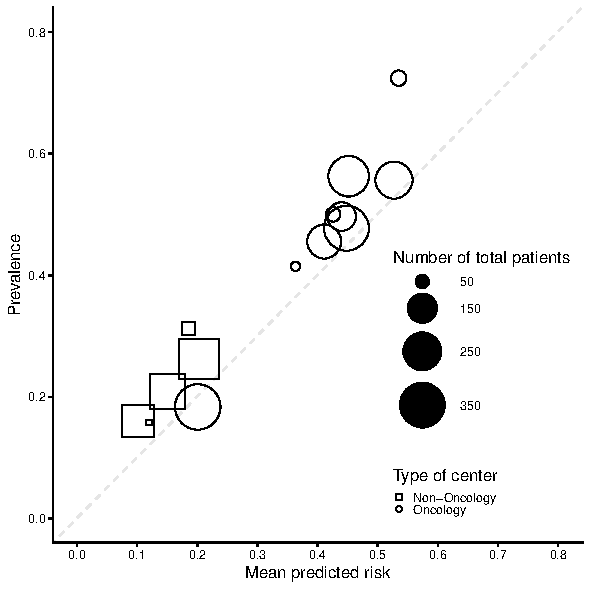
\includegraphics[width=0.8\textwidth]{figures/ClusteredCalibration/F1.pdf}
\caption[Mean predicted risk of ADNEX and prevalence across 14 centers]{Prevalence and mean predicted ADNEX risk by center across the 14 centers in the dataset. The dashed diagonal line indicates perfect calibration.}
\label{fig:4:1}
\end{figure}

\subsection{Notation}
We assume to have a dataset with a total of \emph{J} clusters and use \(j = (1,\ldots,J)\) to index the clusters. In each cluster, we have \(n_{j}\) patients and we index the patients using \(i = \left( 1,\ldots,n_{j} \right)\). The total sample size is \(N = \sum_{j = 1}^{J}n_{j}\)\emph{.} We use \(y_{ij} \in 0,1\) to denote the outcome of patient \(i\) in cluster \(j\), which takes on the value 0 in case of a non-event and 1 in case of an event. We assume that \(y_{ij}\) follows a Bernoulli distribution \(y_{ij} \sim \text{Bern}\left( \pi_{ij} \right)\), where \(\pi_{ij}\) denotes the probability of experiencing the event. Typically, \(\pi_{ij}\) is expressed as a function of a set of risk characteristics, captured in the covariate vector \(\mathbf{x}_{ij}\) and we assume that there exists an unknown regression function \(r\left( \mathbf{x}_{ij} \right) = P\left( y_{ij} = 1 \middle| \mathbf{x}_{ij} \right)\). We approximate this function using a risk prediction model, where we model the outcome as a function of the observed risk characteristics and employ statistical or machine learning techniques to estimate this model. A general expression that encompasses both types is

\begin{equation}{r}
\text{P}\left( y_{ij} = 1\mid\mathbf{x}_{ij} \right) = \pi\left( \mathbf{x}_{ij} \right) = f\left( \mathbf{x}_{ij} \right)\
\label{eq:3:1}
\end{equation}

Where \(f( \cdot )\) denotes the predicted risk given covariate vector \(\mathbf{x}_{ij}\). In a logistic regression model, we have that

\[\pi\left( \mathbf{x}_{ij} \right) = \frac{e^{\mathbf{x}_{ij}^{T}\mathbf{\beta}}}{1 + e^{\mathbf{x}_{ij}^{T}\mathbf{\beta}}}\]

where \(\mathbf{\beta}\) denotes the parameter vector. We can rewrite the above equation to

\[{{\ \ \ \log}\left( \frac{\pi\left( \mathbf{x}_{ij} \right)}{1 - \pi\left( \mathbf{x}_{ij} \right)} \right) = \mathbf{x}_{ij}^{T}\mathbf{\beta}}{\text{logit}\left( \pi\left( \mathbf{x}_{ij} \right) \right)\mathbf{=}\mathbf{x}_{ij}^{T}\mathbf{\beta}}\]

We can employ splines to allow for a non-linear relationship between the covariates and outcome \cite{harrellRegressionModelingStrategies2015}. To estimate equation \ref{eq:3:1}, we fit a statistical or machine learning model to the training data. The resulting model fit then provides us with the predicted probability \(\widehat{\pi}\left( \mathbf{x}_{ij} \right)\).

Using calibration curves, we examine how well the predicted probabilities correspond to the actual event probabilities \cite{steyerbergClinicalPredictionModels2019a,vancalsterCalibrationHierarchyRisk2016,dimitriadisHonestCalibrationAssessment2023,decockcampoReliablePredictiveAnalytics2023}. A calibration plot maps the predicted probabilities \(\widehat{\pi}\left( \mathbf{x}_{ij} \right)\) to the actual event probabilities \(\text{P}\left( y_{ij} = 1\mid\widehat{\pi}\left( \mathbf{x}_{ij} \right) \right)\ \)and hereby provides a visual representation of the alignment between the model's estimated risks and the true probabilities. For a perfectly calibrated model, the calibration curve follows the diagonal as \(\text{P}\left( y_{ij} = 1\mid\widehat{\pi}\left( \mathbf{x}_{ij} \right) \right)\  = \pi\left( \mathbf{x}_{ij} \right)\) for all \(i\).

\subsection{Flexible calibration plots ignoring clustering}
We can estimate the calibration curve using a logistic regression model \cite{decockcampoReliablePredictiveAnalytics2023,onbehalfoftopicgroupevaluatingdiagnostictestsandpredictionmodelsofthestratosinitiativeCalibrationAchillesHeel2019,coxTwoFurtherApplications1958}

\[\text{logit}\left( \text{P}\left( y_{ij} = 1\mid\widehat{\pi}\left( \mathbf{x}_{ij} \right) \right) \right)\mathbf{=}\alpha + \zeta\ \text{logit}\left( \widehat{\pi}\left( \mathbf{x}_{ij} \right) \right)\]

where we estimate the observed proportions as a function of the (logit transformed) predicted probabilities. Using the fitted model, we create a calibration curve by plotting the \(\widehat{\pi}\left( \mathbf{x}_{ij} \right)\) against the observed proportions \(\widehat{P}\left( y_{ij} = 1\mid\widehat{\pi}\left( \mathbf{x}_{ij} \right) \right)\). This model, however, only allows for a linear relationship and, as such, does not adequately capture moderate calibration. To allow for a non-linear relationship between \(\widehat{\pi}\left( \mathbf{x}_{ij} \right)\) and \(y_{ij}\), we can rely on non-parametric smoothers, such as locally estimated scatterplot smoothing (loess) or restricted cubic splines

\[\text{logit}\left( \text{P}\left( y_{ij} = 1\mid\widehat{\pi}\left( \mathbf{x}_{ij} \right) \right) \right)\mathbf{=}s\left( \text{logit}\left( \widehat{\pi}\left( \mathbf{x}_{ij} \right) \right) \right).\]

Here, \(s( \cdot )\) denotes the smooth function applied to the logit transformed predicted probability. This results in a flexible calibration plot, which is implemented in R packages such as CalibrationCurves (val.prob.ci.2 function), rms (val.prob function), or tidyverse (cal\_plot\_logistic function) \cite{vancalsterCalibrationHierarchyRisk2016,harrellRegressionModelingStrategies2015,wickhamWelcomeTidyverse2019,rcoreteamLanguageEnvironmentStatistical2024}.

Figure~\ref{fig:4:2} presents a flexible calibration curve (using a restricted cubic spline) based on the motivating example with pooled data, and the results of a grouped calibration assessment for ovarian malignancy prediction. The panel below shows the sample distribution of the estimated risks for benign cases (blue) and malignant cases (red). The plots suggest that risks were estimated too low.

\begin{figure}
\centering
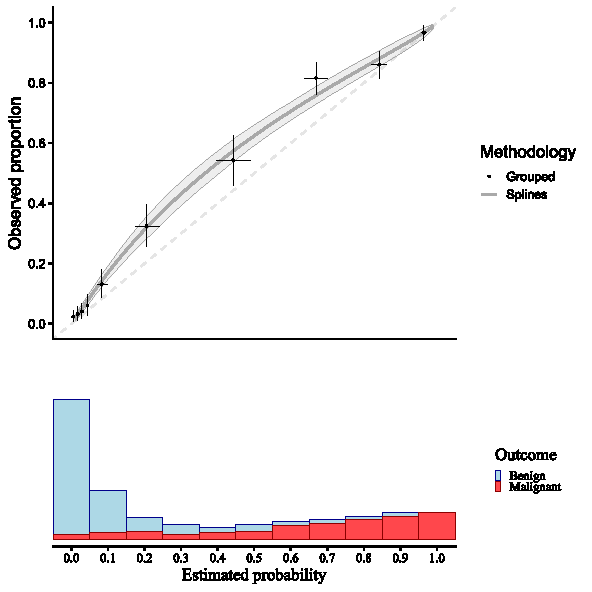
\includegraphics[width=0.8\textwidth]{figures/ClusteredCalibration/F2.pdf}
\caption[Traditional flexible calibration plots and risk distributions]{Traditional flexible calibration curves for the ADNEX model in the motivating example. Observed proportion is estimated with a logistic model with restricted cubic splines to model non-linear effects, and estimated risks are grouped in 10 groups. Confidence intervals are shown for 1000 bootstraps with a shaded area for splines and a + for grouped calibration. The dashed diagonal line indicates perfect calibration.}
\label{fig:4:2}
\end{figure}

Since there is no commonly accepted way to estimate calibration curves for prediction models in clustered data, we present three approaches covering different statistical methodologies. First, we present a grouped clustered calibration plot based on a bivariate random effects meta-analysis model (Clustered Group Calibration; \gls{CGC}). Second, we introduce a two-stage univariate random effects meta-analytical approach for the estimation of the observed events (Two-stage meta-analysis calibration; \gls{TMAC}). Finally, we provide a one-step approach where we fit a random effects model with smooth effects to obtain individual calibration slopes per cluster (Mixed model calibration; \gls{MIXC}). We present the summary of the three proposed approaches in Table~\ref{tab:4:1}.

\begin{table}
\centering
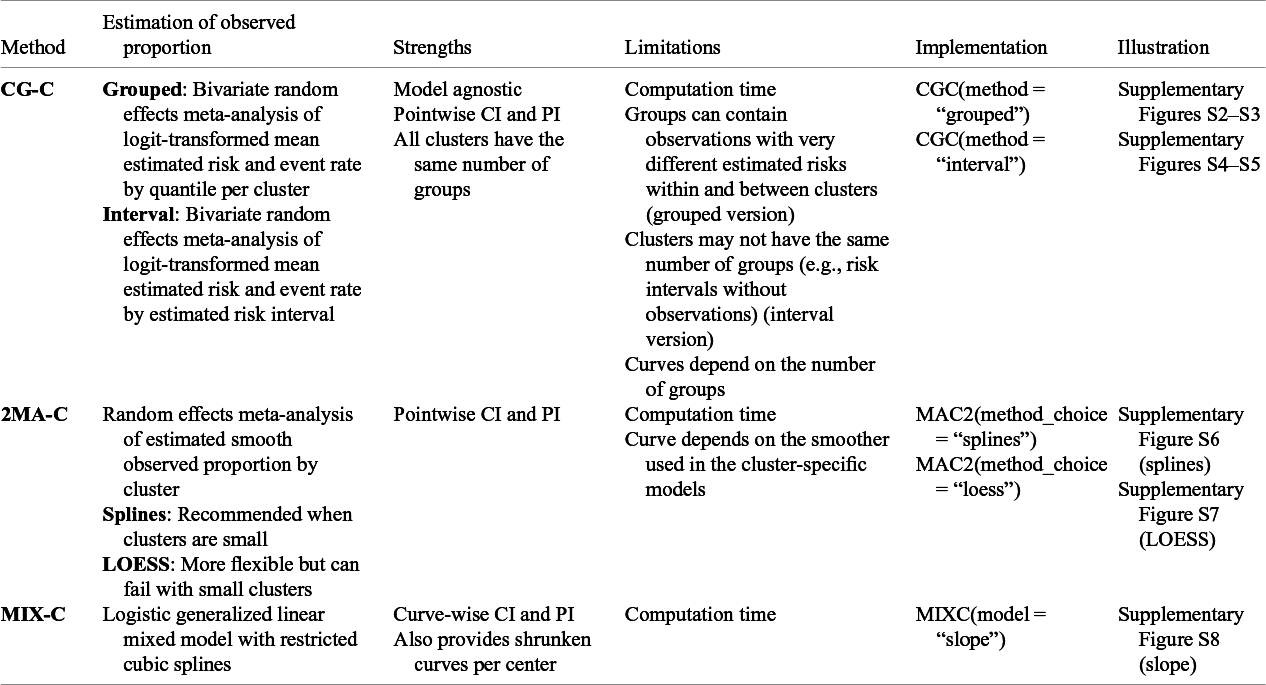
\includegraphics[width=1\textwidth]{figures/ClusteredCalibration/T1.png}
\caption[Overview introduced methods]{Overview of introduced methodologies for creating flexible calibration curves accounting for clustering.}
\label{tab:4:1}
\end{table}

\subsection{Clustered group calibration (CG-C)}
The \gls{CGC} approach is a two-stage approach that extends the traditional grouped calibration approach to clustered data. In the traditional approach, data is pooled and groups are created based on quantiles (often deciles). In \gls{CGC}, we create \(Q\) quantiles in every cluster (based on the estimated risk distribution per cluster) with \(q = (1,\ldots,Q)\). Hereafter, we pool the estimated risks and observed proportions with a bivariate random effects meta-analysis at each quantile \(q\). The logit-transformed observed proportion and average estimated risk are the response variables and we capture the cluster-specific deviation by including a random intercept. The equation of this model is given by

\begin{equation}{r}
\genfrac{[}{]}{0pt}{}{\text{logit(}{\overline{y}}_{qj})}{\text{logit(}{\overline{\widehat{\pi}}}_{qj})} = \genfrac{[}{]}{0pt}{}{{{}_{\overline{y}}\mu}_{q} + u_{qj} + \varepsilon_{qj}}{{_{\overline{\widehat{\pi}}}^{}\mu}_{q} + \nu_{qj} + \epsilon_{qj}}
\end{equation}

where \({\overline{y}}_{qj}\) denotes the prevalence of cluster \(j\) within quantile \(q\) and \({\overline{\widehat{\pi}}}_{qj}\) the average estimated risk in cluster \(j\) within quantile \(q\). We use the subscript \(q\) in the quantities to indicate that this refers to quantile \(q\). \(u_{qj}\) and \(\nu_{qj}\) represent the random intercepts for cluster \(j\), capturing the between-cluster heterogeneity whereas \(\varepsilon_{qj}\) and \(\epsilon_{qj}\) account for the within-cluster error. In this model, we assume that \({{}_{\overline{y}}\mu}_{q} + u_{qj}\) and \({_{\overline{\widehat{\pi}}}^{}\mu}_{q} + \nu_{qj}\) are randomly drawn from a distribution with mean (or pooled) \({{}_{\overline{y}}\mu}_{q}\) and \({_{\overline{\widehat{\pi}}}^{}\mu}_{q}\), respectively. Additionally, we assume that

\[\begin{bmatrix}
u_{qj} \\
\nu_{qj}
\end{bmatrix} \sim \mathcal{N}\left( \genfrac{[}{]}{0pt}{}{0}{0},\Omega_{q} \right)\ and\ \begin{bmatrix}
\varepsilon_{qj} \\
\epsilon_{qj}
\end{bmatrix} \sim \mathcal{N}\left( \genfrac{[}{]}{0pt}{}{0}{0},\Sigma_{qj} \right)\]

where \(\Omega_{q}\) and \(\Sigma_{qj}\) represent the between-cluster and within-cluster covariance matrices within quantile \emph{q}, respectively.

\[\Omega_{q} = \begin{bmatrix}
{}_{\overline{y}}\tau_{q}^{2} & {}_{b}\rho_{q} \; {}_{\overline{y}}\tau_{q} \; {}_{\overline{\widehat{\pi}}}\tau_{q} \\
{}_{b}\rho_{q} \; {}_{\overline{y}}\tau_{q} \; {}_{\overline{\widehat{\pi}}}\tau_{q} & {}_{\overline{\widehat{\pi}}}\tau_{q}^{2}
\end{bmatrix}\]

\[\Sigma_{qj} = \begin{bmatrix}
{}_{\overline{y}}\sigma_{qj}^{2} & {}_{w}\rho_{q} \; {}_{\overline{y}}\sigma_{qj} \; {}_{\overline{\widehat{\pi}}}\sigma_{qj} \\
{}_{w}\rho_{q} \; {}_{\overline{y}}\sigma_{qj} \; {}_{\overline{\widehat{\pi}}}\sigma_{qj} & {}_{\overline{\widehat{\pi}}}\sigma_{qj}^{2}
\end{bmatrix}\]

We use \({}_{\overline{y}}\sigma_{qj}^{2}\) and \({}_{\overline{\widehat{\pi}}}\sigma_{qj}^{2}\) to denote the variance of \({\overline{y}}_{qj}\) and \({\overline{\widehat{\pi}}}_{qj}\), \({}_{w}\rho_{q}\) represents the within-cluster correlation and \({}_{b}\rho_{q}\) the between-cluster correlation in quantile \emph{q}. The between-study variance is denoted as \({}_{\overline{y}}\tau_{q}^{2}\) and \({}_{\overline{\widehat{\pi}}}\tau_{q}^{2}\). For each quantile \emph{q,} we use a bivariate meta-analysis model to account for the strong dependence between the average estimated risk and observed proportion. The calibration plot is then created by plotting the \(Q\) values of \({}_{\overline{\widehat{\pi}}}\hat{\mu}_{q}\) on the x-axis and the \({}_{\overline{y}}\hat{\mu}_{q}\) on the y-axis. This approach has the advantage of obtaining an observed proportion per cluster in a model-agnostic way. In addition, it provides uncertainty measures in the cluster with the average random effect with confidence intervals for that effect and in a hypothetical new cluster (\gls{PI}; prediction intervals). It also has some limitations. First, it has the same drawback as the traditional grouped calibration because the curve is dependent on the number of quantiles selected, especially when the sample size is limited. Second, and linked to the previous limitation, the arbitrary selection of \(Q\) quantiles might create groups that are too heterogeneous between clusters because the estimated risks distributions differ (e.g. a high risk setting vs a low risks setting). Third, the meta-analysis does not provide cluster-specific curves using empirical Bayes. We used the rma.mv function of the metafor package \cite{viechtbauerConductingMetaanalysesMetafor2010a}.

We include an extension to the proposed methodology that we call ``interval'' grouping. The methodology is the same except for the way the groups are created. Per cluster, we create \emph{I} groups by dividing the probability space (0-1) into \emph{I} equally spaced intervals\emph{.} In this way, we will create \emph{I} groups of different sizes based on the estimated risks. By doing this, we reduce the within group variability at the expense of not having necessarily all clusters present in all \emph{I} groups. The algorithm, additional details on the implementation and illustration are available in the Supporting material (Appendix A1, Figure S2-S5) and code for the implementation in the \gls{OSF} repository \cite{barrenadaOSFClusteredFlexible2024}. 

\subsection{Two-stage meta-analysis calibration (2MA-C)}
For the second approach, we use a two-stage random effects meta-analysis to estimate the calibration plot. First, we fit a flexible curve per cluster with a smoother of choice. Currently, we have implemented restricted cubic splines and LOESS. For LOESS, in each cluster, the span parameter with the lowest bias-corrected AIC is selected. For restricted cubic splines, the number of knots per cluster is selected by performing a likelihood ratio test between all combinations of models with 3,4, and 5 knots, selecting the model with the least knots that provides the best fit. We train a flexible curve per cluster and estimate the observed proportion for a fixed grid of estimated risks from 0.01 to 0.99 (\(G\), default is 100 points). Hereafter, we use a random effects meta-analysis model per point in the grid to combine the logit-transformed predictions across clusters, fitting the following univariate model per point \(g\) in the grid.

\[\text{logit}({}_{s}\widehat{\pi}_{gj}) = {}_{\widehat{\pi}}\mu_{g} + \nu_{gj} + \epsilon_{gj}.\]

\({}_{s}\widehat{\pi}_{gj}\) denotes the predicted proportion of point \(g\) for cluster \(j\), \({}_{\widehat{\pi}}\mu_{g}\) the overall mean for point \(g\), \(\nu_{gj}\) the cluster-specific deviation and \(\epsilon_{gj}\) the error. We assume that \(\nu_{gj} \sim \mathcal{N}\left( 0, {}_{\widehat{\pi}}\tau_{g}^{2} \right)\) and \(\epsilon_{gj} \sim \mathcal{N}\left( 0, {}_{\widehat{\pi}}\sigma_{gj}^{2} \right)\). Further, we include the inverse of the variance of \(\text{logit}({}_{s}\widehat{\pi}_{gj})\) as weight and hereby take both the cluster-specific (\({}_{\widehat{\pi}}\sigma_{gj}^{2}\)) and between-cluster variability (\({}_{\widehat{\pi}}\tau_{g}^{2}\)) into account. As such, clusters with more precise estimates are assigned greater weights. This approach has the strength of being easy to compute and providing heterogeneity measures for the cluster with average calibration. This allows to plot confidence and prediction intervals which help to visually assess the certainty of the average curve (\gls{CI}) and the heterogeneity between hypothetical new clusters (\gls{PI}) in the whole range of predicted probabilities. The main limitation is that it is based on the smoothing technique used in each individual cluster so the curves will vary depending on the smoother selected. Additionally, the technique treats each point in the grid as independent, leading to pointwise confidence and prediction intervals. Cluster-specific curves are obtained in the first stage independently from the rest of the clusters. The algorithm, additional details on the implementation and illustration are available in the Supporting material (Appendix A2, Figure S6-S7) and code for the implementation in the \gls{OSF} repository.

\subsection{Mixed model calibration (MIX-C)}
In the third approach, we employ a one-stage logistic generalized linear mixed model (\gls{GLMM}) to model the outcome as a function of the logit-transformed predictions. To allow for a non-linear effect, we employ restricted cubic splines with three knots for both the fixed and random effects

\[\text{logit}\left( \text{P}\left( y_{ij} = 1\mid\widehat{\pi}\left( \mathbf{x}_{ij} \right),\widetilde{s_{j}} \right) \right)\  = \ s\left( \text{logit}\left( \widehat{\pi}\left( \mathbf{x}_{ij} \right) \right) \right)\  + \ \widetilde{s_{j}}\left( \text{logit}\left( \widehat{\pi}\left( \mathbf{x}_{ij} \right) \right) \right).\]

Here, \(\widetilde{s_{j}}\) denotes the smooth random effect for cluster \(j\). The model is fit using lme4 \cite{batesFittingLinearMixedEffects2015} and splines are added with rms package \cite{harrelljrRmsRegressionModeling2009}. This approach estimates the calibration per cluster and the variance of the random effects in a single step. As opposed to the random effects in \gls{TMAC}, the \gls{MIXC} model takes all observations across the entire spectrum of predicted risk into account when predicting the realized values of the random effects and cluster-specific calibration curves. The main limitation is the computation time needed when the number of clusters is large. The algorithm, additional details on the implementation, and illustration are available in the Supporting material (Appendix A3, FigureS8), and code for the implementation is available in the \gls{OSF} repository \cite{barrenadaOSFClusteredFlexible2024}.

\subsection{Results for the case example}
A visual analysis of the different curves shows that all the approaches present similar results on the case example, in line with the previously obtained results ignoring clustering (Figure~\ref{fig:4:3}). All plots suggest that \gls{ADNEX} overestimated risks. Nevertheless, there are important differences in the estimated uncertainty and heterogeneity. Details, visualizations, and variations of each method are shown in Figures S2-S8. The methods will be available in the CalibrationCurves package from version 2.0.0 onwards \cite{decockCalibrationCurvesPackageAssessing2023}.

\begin{figure}
\centering
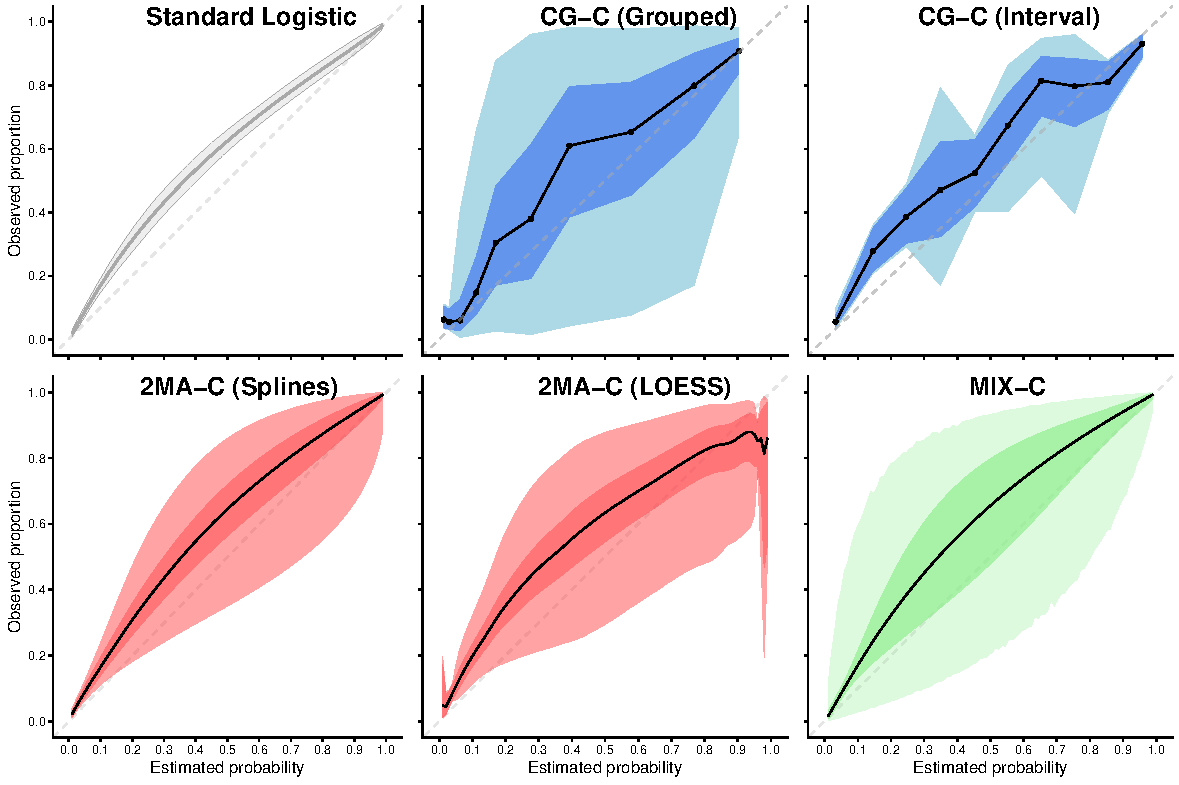
\includegraphics[width=1\textwidth]{figures/ClusteredCalibration/F3.pdf}
\caption[Comparison of traditional plots and introduced methododologies]{Comparison of the standard logistic regression with splines and the three introduced methodologies with CI (bright shaded) and PI (light shaded). Number of quantiles for CG-C were 10, 2MA-C fitted center-specific curves with splines or LOESS, and MIX-C used random intercept and slopes with restricted cubic splines and three knots. The dashed diagonal line indicates perfect calibration.}
\label{fig:4:3}
\end{figure}

\section{Simulation study}
The motivating example showcases the applicability of the methods. However, with real data it is not possible to know the true underlying observed proportion. Therefore, we designed a simulation study to explore the performance of the introduced approaches and compare it with cluster ignorant methodologies.

\subsection{Methods}
The data generating models were based on logistic regression with a random intercept per cluster, hence the formula to obtain the true probabilities was of the form \(\text{logit}\left( \pi\left( x_{ij} \right) \right)\mathbf{=}\beta_{0} + x_{ij}\beta_{1}\mathbf{+}u_{j}\). \(\beta_{0}\) represents the intercept, \(\beta_{1}\) the corresponding effect of covariate \(x\) and \(u_{j}\) is the cluster-specific deviation. We first obtain the true models according to a full factorial design where two factors were varied: little vs strong clustering (\gls{ICC} 5\% or 20\%) and lower vs higher true area under the receiver operating characteristic curve (\gls{AUC};0.75 and 0.9). Event rate was fixed at 30\% for the whole population but varied between clusters according to the variance of the random intercept \(u_{j}\). For each data generating mechanism, we generated data for 200 clusters and 2.000.000 patients (10.000 observations per cluster) and a single normally distributed linear predictor (\(x\)\emph{,} which can be seen as a combination of several predictors) with mean 0 and variance 1. Random effects (\(u_{j})\ \)were also normally distributed with variance according to the desired \gls{ICC}. \gls{ICC} is calculated as the variance of a null random intercept model divided by the total variance, calculated as the addition of the variances of the null random intercept model and the standard logistic distribution \cite{hosmerAppliedLogisticRegression2013a}. \gls{AUC} was controlled by varying the coefficient (\(\beta_{1}\)) and the desired event rate was controlled by modifying the intercept \(\beta_{0}\). We obtained 4 superpopulations by trial and error (Table S1). The code to obtain the superpopulations is available in the \gls{OSF} repository.

In each of the superpopulations we draw 4 scenarios, inspired by real validation or development studies, varying events per cluster (\gls{EPC}) (20 vs 200) and number of clusters (5 vs 30). These scenarios refer to the dataset on which hypothetical prediction models are developed or validated. This results in 16 scenarios overall, by combining all values for \gls{ICC}, \gls{AUC}, \gls{EPC} and number of clusters. We then applied the methods for varying development or varying validation sample size.

\subsubsection{Varying development size}
The clusters and patients within each cluster were selected randomly and the number of patients was selected according to the prevalence and the desired \gls{EPC} (\(n_{j}\) = \gls{EPC} * 1.15 divided by cluster prevalence, we multiply \gls{EPC} to ensure that the desired \gls{EPC} is obtained across all clusters). We developed logistic regression models with restricted cubic splines and 3 knots in these training datasets. Then, we externally validated the calibration of the model in patients from clusters not used for model development in an ideal situation with high number of clusters and high \gls{EPC}. Therefore, we validated models on a random selection of 100000 observations from a random selection of 30 clusters that were not sampled for model development. On average, each cluster contained 1000 events and 3333 observations, but the number of events varied depending on the cluster specific event rate.

\subsubsection{Varying validation size}
Additionally, we validate the models with varying validation sample size. In this case we fixed the model to be validated to a logistic regression model with restricted cubic splines and 3 knots trained with a sufficiently large sample size according to Riley's criteria (N = 1711) from a cluster with average event rate in each of the superpopulations \cite{rileyMinimumSampleSize2021}. Then we validated those models varying \gls{EPC} (20 vs 200) and number of clusters (5 vs 30) in the validation sample.

We applied the \gls{CGC} (grouped and interval), \gls{TMAC} (splines and loess) and \gls{MIXC} approaches to the validation sample in both approaches. For comparison, we also obtained a standard flexible logistic calibration model (i.e. ignoring clustering, see section 2.3) using restricted cubic splines and 3 knots. True risks are obtained using the formula in Table S1, and the true risks in the cluster with the average effect are obtained by setting the random intercept to 0. These true risks can be used to generate true calibration curves per cluster and for the cluster with the average effect. To numerically compare the deviation of the estimated calibration curve from the true one, we calculate the mean squared calibration error (\gls{MSCE}) as the mean squared difference between the estimated observed proportions and the true observed proportions (based on the true risks) in the cluster with the average effect (setting \(u_{j} = 0\)) over a fixed grid of 100 estimated risks (100 evenly spaced points from 0.01 to 0.99) \cite{vanhoordeSplinebasedToolAssess2015}. For \gls{CGC}, the grid contains 10 points by definition. The process was repeated 100 times per scenario.

\subsubsection{Heterogeneity}
We evaluated the coverage of the 95\% prediction intervals. For each of the three methods, using the same grid of values that we used for the \gls{MSCE}, we evaluated whether the true cluster-specific risk (including random effects) falls within the prediction interval at each of the grid points. This means that we obtained the true cluster specific probabilities using the formula in Table S1 and compared for each clustered calibration approach if the prediction interval contained the true values. Coverage was calculated as the proportion over the 200 clusters in the superpopulations.

\subsection{Results}
The median \gls{MSCE} results for varying validation sample size are displayed in Table~\ref{tab:4:2} (multiplied by 100) and Figure~\ref{fig:4:4}. Note that \gls{CGC} focuses on 10 points whereas the other approaches focus on a grid of 100 points, such that \gls{CGC} and the other approaches are not directly comparable. \gls{MIXC} was the best performing approach in all cases. \gls{TMAC} (splines) also performed well in scenarios with high validation sample size. In general, the \gls{MSCE} was better with high \gls{EPC}, low \gls{ICC} and with more clusters in the validation. Standard flexible logistic calibration performed considerably worse in all scenarios, in particular when \gls{ICC} was high. When evaluated on a big validation sample with varying development size the results showed also that \gls{TMAC} (splines) and \gls{MIXC} were the best methods across all scenarios (Table~\ref{tab:4:3} and Figure S9).

\begin{table}
\centering
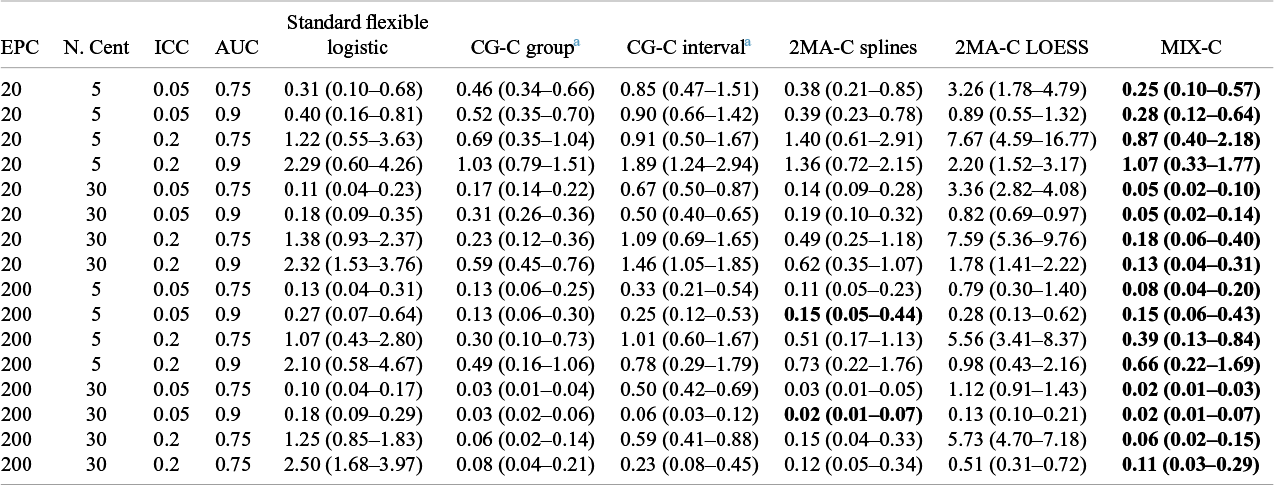
\includegraphics[width=1\textwidth]{figures/ClusteredCalibration/T2.png}
\caption[Median MSCE for varying validation sample size]{Median (IQR) squared difference between true average probabilities and estimated observed proportion (MSCE) with logistic calibration, CG-C (10 groups), 2MA-C, and MIX-C methods for a logistic model varying validation events per center and number of centers. Bold numbers indicate best performance across approaches. MSCE is multiplied by 100.}
\label{tab:4:2}
\end{table}

\begin{figure}
\centering
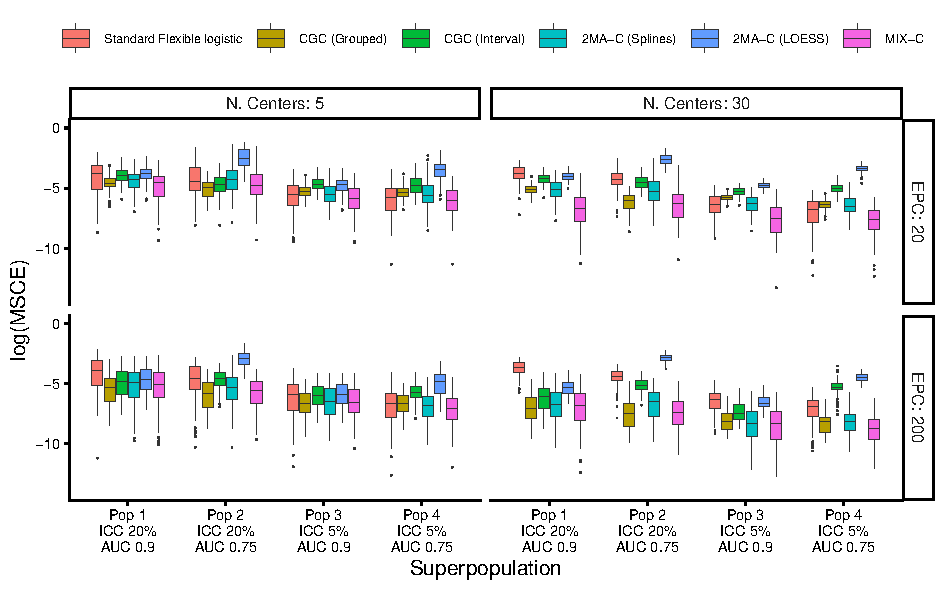
\includegraphics[width=1\textwidth]{figures/ClusteredCalibration/F4.pdf}
\caption[Boxplots of mean squared calibration error]{Boxplots of mean squared calibration error (log) for fixed prediction models varying validation events per center (EPC) and the number of centers in the validation.}
\label{fig:4:4}
\end{figure}

\begin{table}
\centering
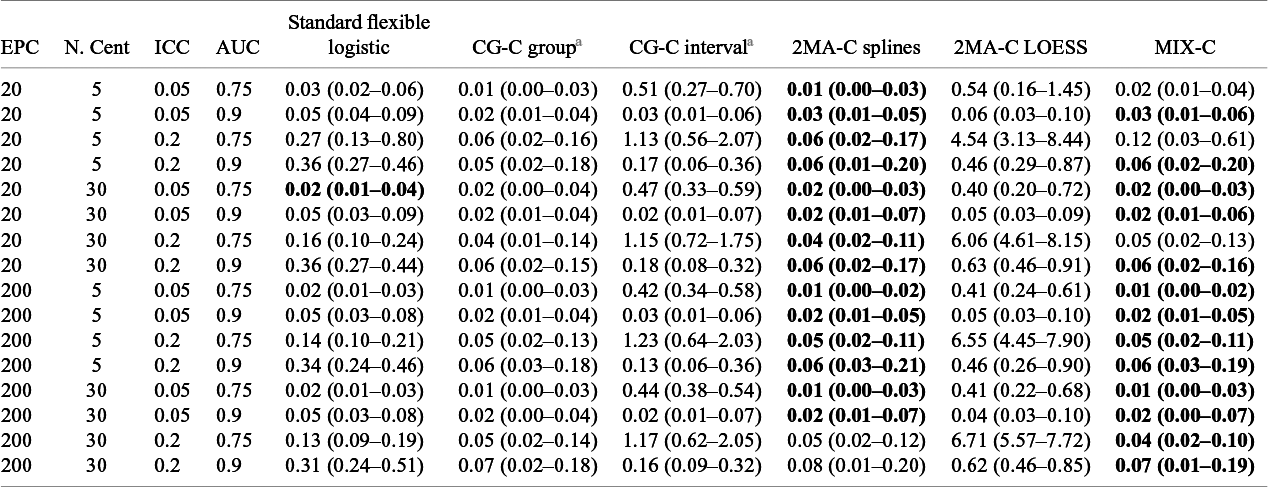
\includegraphics[width=1\textwidth]{figures/ClusteredCalibration/T3.png}
\caption[Median MSCE for varying training sample size]{Median (IQR) squared difference between true average probabilities and estimated observed proportion (MSCE) with logistic calibration, CG-C (10 groups), 2MA-C, and MIX-C methods for a logistic model varying training sample events per center and number of centers. Bold numbers indicate best performance across approaches. MSCE is multiplied by 100.}
\label{tab:4:3}
\end{table}

The prediction interval coverage with varying validation sample was close to nominal with high \gls{EPC} and low \gls{ICC} and when using the \gls{TMAC} (splines) approach (Figure~\ref{fig:4:5}). When \gls{EPC} was high the coverage was close to nominal in the region where validation data was available but very poor at the tails (i.e. regions with few validation data) except for the \gls{MIXC} approach. \gls{MIXC} had correct coverage when \gls{ICC} was high and \gls{AUC} low, too wide prediction intervals when \gls{ICC} was low and too narrow \gls{PI} when \gls{ICC} and \gls{AUC} were high. When \gls{EPC} was low, increasing the number of clusters reduced notably the coverage, especially for the grouped approaches and at the tails. The coverage in the large validation dataset was poor at tails except for \gls{MIXC} (Figure S10). High \gls{AUC} and low \gls{ICC} in development tend to have better \gls{PI} coverage.

\begin{figure}
\centering
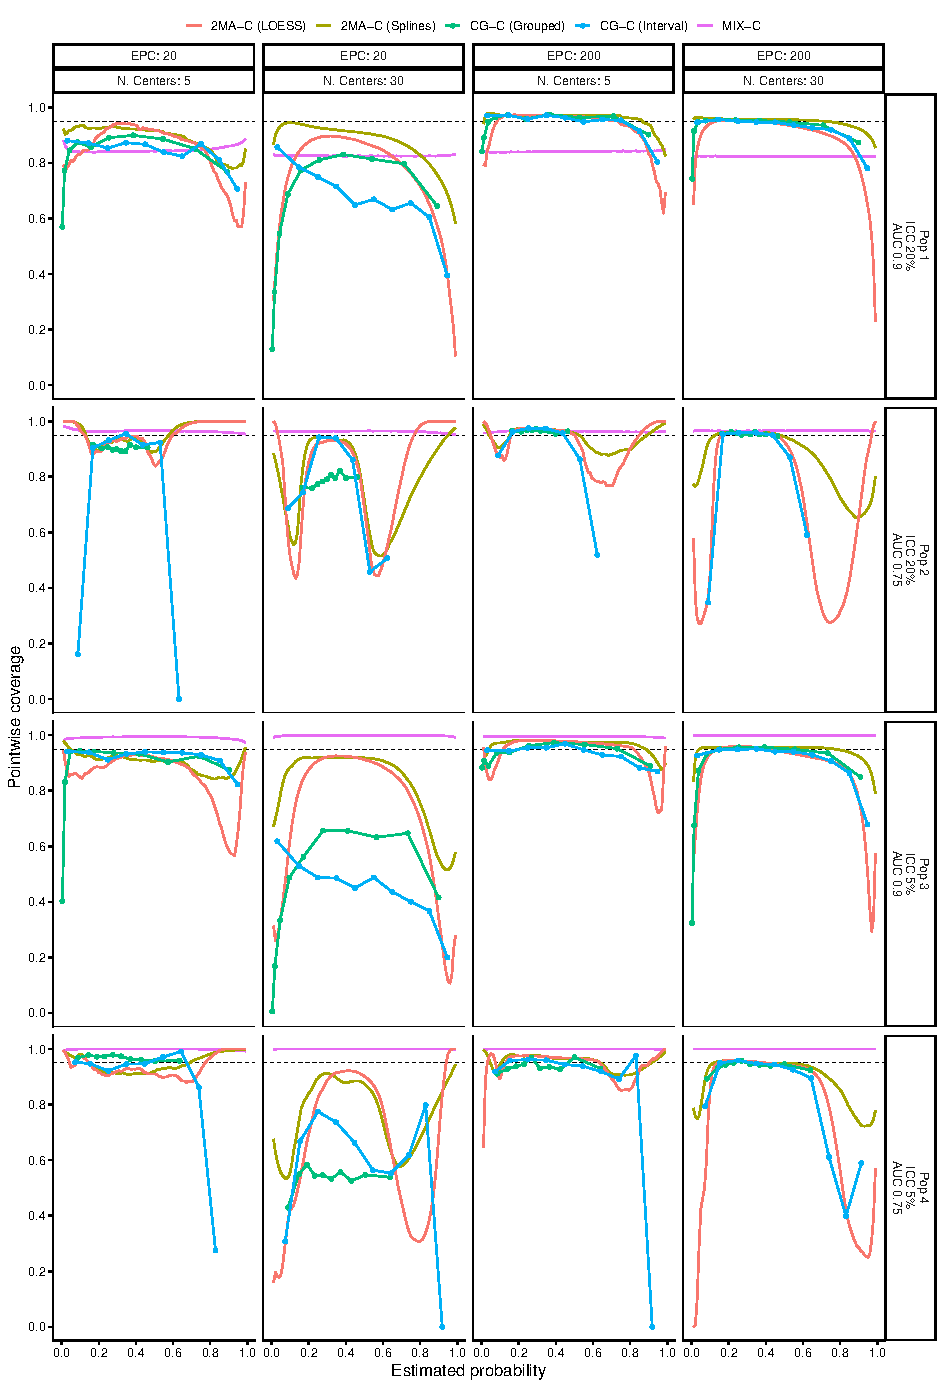
\includegraphics[width=1\textwidth]{figures/ClusteredCalibration/F5.pdf}
\caption[Pointwise prediction interval coverage]{Pointwise prediction interval coverage varying the validation sample size. The model validated is the same in each superpopulation, and it was trained from a center with average event rate and with adequate sample size. The black dotted line indicates nominal coverage (95\%).}
\label{fig:4:5}
\end{figure}

Code and data to reproduce the simulation study and analysis are available in the \gls{OSF} repository \cite{barrenadaOSFClusteredFlexible2024}.

\section{Synthetic data}
The simulation study showed that the methods correctly estimate observed proportions under different logistic \glspl{DGM}. In the real world, the link between outcome and predictors is often not perfectly defined by a linear or logistic function. Therefore, we aim to test the methods in a more flexible situation using a synthetically generated dataset based on the data used in the motivating example.

\subsection{Methods}
To generate synthetic data, we use data from the International Ovarian Tumor Analysis (\gls{IOTA}) consortium that was used to develop prediction models to estimate the risk of malignancy in patients with an ovarian tumor \cite{vancalsterValidationModelsDiagnose2020,vancalsterEvaluatingRiskOvarian2014}. We used the synthpop package in R, which learns the structure of the data and generates a new dataset where individual patient data is masked but the underlying structure is preserved \cite{nowokSynthpopBespokeCreation2016}. We generated synthetic data for 1 million individuals for each of the 10 hospitals separately, and used these synthetic patients as cluster-specific populations (retaining the clustered structure of the original dataset). We generated two true models per center: one based on a logistic regression model with splines for continuous variables, and one based on a random forest model with number of randomly selected parameters per split (mtry) set to three and the depth of the individual trees set to ten (minimum node size) \cite{wrightRangerFastImplementation2017}. Both models were trained on the real data from that center, using the nine \gls{ADNEX} predictors listed above except type of center. The true models were applied to the 1 million synthetic patients, and the outcome was generated with Bernoulli trials based on the true risks of malignancy from the applied models. This means that the same synthetic patient has two true risks and can have two different outcomes. The code to generate the synthetic data is available in the \gls{OSF} repository, but the original data or the synthetic data are not publicly available. The comparison of the real and synthetic data for quality check in one center is presented in Figure S11.

We used the synthetic data to validate the calibration of the published \gls{ADNEX} model without CA125 in each center \cite{vancalsterEvaluatingRiskOvarian2014}. We define 15 scenarios based on the number of centers (2,5,10) and validation data \gls{EPC} (20,100,200,500,1000). We repeat this 1000 times, by randomly drawing validation datasets. If the number of centers was 2 or 5, the centers were randomly chosen as well. In each repetition, we calculate \gls{MSCE} for the two true risks. True center-specific curves are obtained by training flexible calibration models (splines with 5 knots) on all 1 million synthetic patients from that center (Figure~\ref{fig:4:6}). We then compared the center specific estimated observed proportions and the true probabilities per center in a fixed grid of 100 values. The only method that obtains center specific curves borrowing information from other clusters is the \gls{MIXC} method and we compare this to standard flexible calibration with LOESS and restricted cubic splines with 3 knots (Stage 1 of \gls{TMAC}).

\begin{figure}
\centering
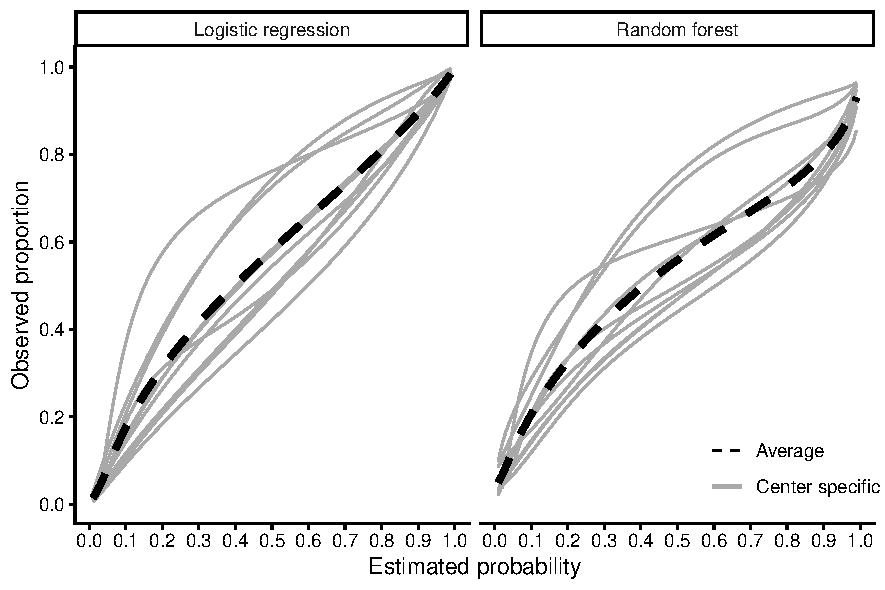
\includegraphics[width=0.8\textwidth]{figures/ClusteredCalibration/F6.pdf}
\caption[Center-specific calibration plots for the synthetic data]{Center-specific (grey) and average true calibration plots for the synthetic data with 1000000 observations per center.}
\label{fig:4:6}
\end{figure}

\subsection{Results}
Median \gls{MSCE} for the synthetic data analysis with 1000 iterations is shown in Table~\ref{tab:4:4} and by center in Figure~\ref{fig:4:7}. \gls{MIXC} was the best performing method in all scenarios when the truth was based on a logistic regression, with splines working equally well in 5 scenarios. When the truth was based on a random forest model \gls{MIXC} was the best with small validation samples (\gls{EPC} < 500) and loess when sample size was above 500 events per center. Borrowing information from other clusters is an example of a bias-variance trade-off and leads to improved accuracy for the estimated cluster-specific curves for clusters with modest sample sizes. Additionally, the performance by approach varied considerably between centers (Figure~\ref{fig:4:7}). That is, the best approach varied by center.

\begin{table}
\centering
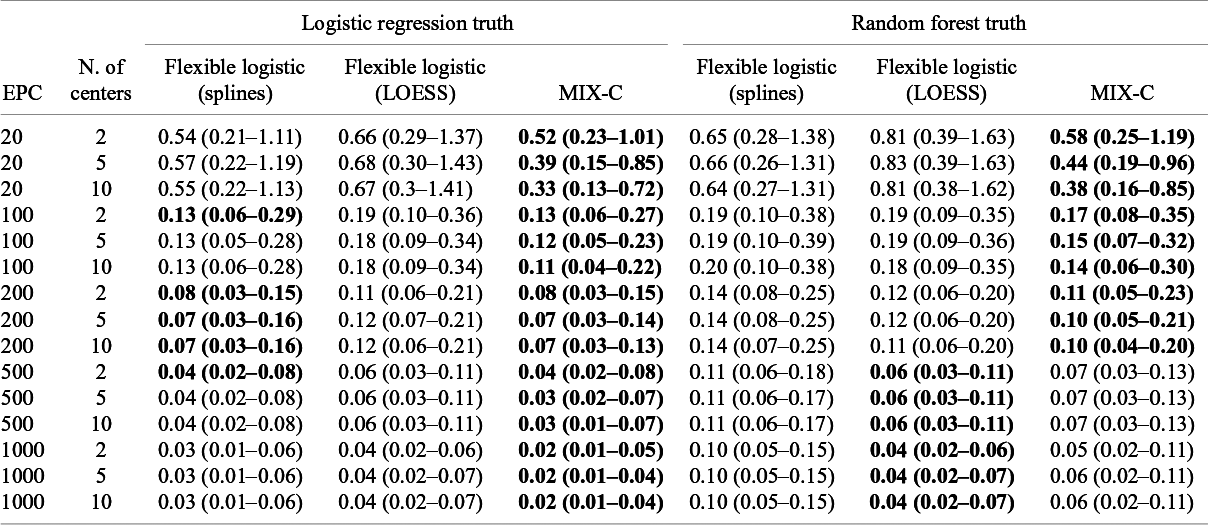
\includegraphics[width=1\textwidth]{figures/ClusteredCalibration/T4.png}
\caption[Median MSCE for center-specific results in the synthetic data]{Median MSCE for the synthetic data study for center-specific results. MSCE is presented multiplied by 100. Bold numbers indicate best performance across approaches.}
\label{tab:4:4}
\end{table}

\begin{figure}
\centering
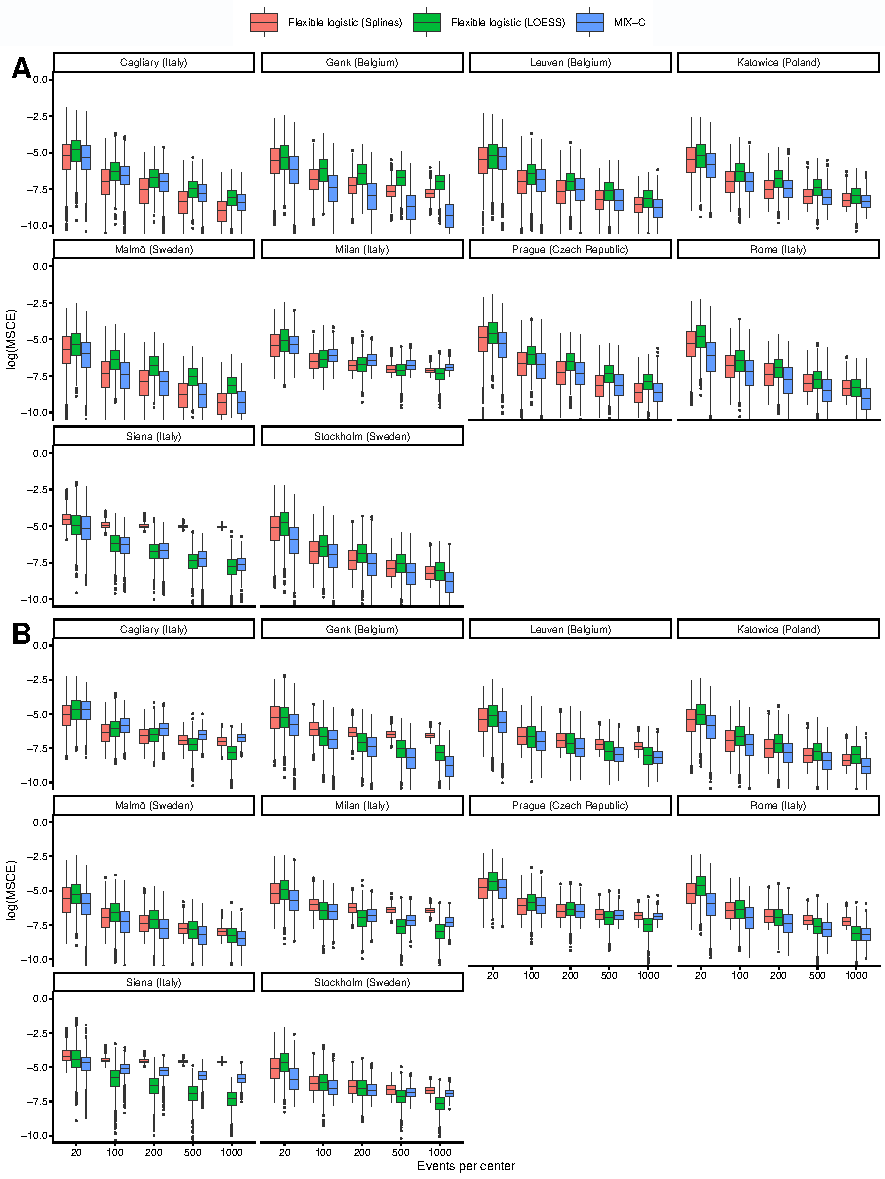
\includegraphics[width=1\textwidth]{figures/ClusteredCalibration/F7.pdf}
\caption[Center-specific log(MSCE) in the synthetic data]{Center-specific results of log(MSCE) by the number of events per center for the logistic truth (a) and the random forest (b) truth.}
\label{fig:4:7}
\end{figure}

\section{Discussion}
Calibration of clinical prediction models is crucial since it is related to the usefulness of the recommended clinical decisions provided by the model \cite{vancalsterCalibrationRiskPrediction2015}. Evaluation of calibration performance is best done with flexible calibration plots \cite{vancalsterCalibrationHierarchyRisk2016,austinGraphicalAssessmentInternal2014}. In this work, we introduced three methods for obtaining flexible calibration plots that account for clustering in the dataset. The first method extended the grouped calibration plot using bivariate random effects meta-analysis (\gls{CGC} method), the second method was a two-step approach in which flexible cluster-specific plots were combined through random effects meta-analysis. We generated cluster-specific plots in two ways: using restricted cubic splines (\gls{TMAC} splines) or LOESS (\gls{TMAC} loess). The third method used a mixed effects logistic calibration model using restricted cubic splines and random intercepts and slopes per cluster (\gls{MIXC}). Through a simulation study and a study using synthetic data from patients with an ovarian tumor, we observed that \gls{MIXC} and \gls{TMAC} (splines) work best to obtain the calibration plot in the cluster with the average effect (simulation study) and \gls{MIXC} for the cluster specific calibration plots (synthetic data). The coverage probability of the prediction interval was suboptimal for all methods and all scenarios with \gls{TMAC} (splines) standing out as the best across scenarios. A disadvantage of \gls{TMAC} (splines) is that the estimated calibration curves per cluster deviated more from the true curves per cluster than those obtained by \gls{MIXC}, which uses shrinkage to obtain better cluster-specific calibration curves. While \gls{CGC} may work well too to obtain a calibration plot in the cluster with the average effect when using 10 groups based on deciles, it worked poorly when using 10 groups based on equal intervals of the estimated risk. However, the grouped approach tends to depend on the number and types of groups, which is undesirable \cite{vancalsterPerformanceEvaluationPredictive2024,arrieta-ibarraMetricsCalibrationProbabilistic2022}. Obviously, the other methods depend on the level of smoothing of the spline or LOESS, but we automatically selected these parameters based on statistical goodness of fit to reduce the modeler's choices. We recommend using \gls{TMAC} (splines) to estimate the curve with the average effect and the 95\% \gls{PI} and \gls{MIXC} for the cluster specific curves, especially when sample size per cluster is limited. In our simulation, \gls{TMAC} (loess) had the worst performance possibly due to the logistic data generation mechanism. In real world the association of outcome and predictors tends to be more complex therefore a more flexible approach could be useful, as shown in the synthetic data with a nonlinear data generating mechanism and large validation sample sizes per cluster. In this work we used the method only for external validation, but the methods also apply to model development with clustered data to explore between-cluster calibration heterogeneity during internal-external validation. We provide ready-to-use R functions to plot the curves and obtain numerical results in the \gls{OSF} Repository , and they will soon be incorporated into the ``CalibrationCurves'' package in CRAN \cite{DeCock2023}.

Munoz and colleagues developed similar methodologies to derive calibration plots in large clustered datasets (preprint published after our initial submission) \cite{munoz2025}. In their work they present four approaches to obtain overall calibration plots. Although their rationale is similar to ours in some cases, the implementation is different. The stacking approach is similar to what we define as flexible curve ignoring clustering (section 2.3), where all the data from different clusters is combined into a single dataset and a calibration model is fitted. Their ``One-step meta-analysis'' approach corresponds to our \gls{MIXC} method where a mixed model is fitted. Their ``two step meta-analysis'' method is similar to \gls{TMAC} but they also present a variant where instead of fitted probabilities the model parameters are aggregated. Finally, they introduced an approach where the calibration model is a Generalized Estimating Equation. None of the methodologies include the estimation of prediction intervals. The work is illustrated with an evaluation of a model to diagnose deep vein thrombosis, but no simulation study is included to evaluate the performance of the methodologies or to compare to our results.

The main strength of our methodologies is the inclusion of a heterogeneity measure through the prediction intervals. These intervals indicate, for every estimated risk, the range within which the observed proportion may fall in a new cluster. It is crucial to differentiate the calibration in the cluster with the average effect with the cluster-specific calibration represented in the \glspl{PI}. Whilst a model can be well calibrated in the cluster with the average effect, this does not necessarily imply that the model is perfectly calibrated in every individual cluster. Statements such as ``the model was well calibrated'' based on the cluster with the average effect calibration plot should be avoided, or at least accompanied by a clarification that this only applies to the summary curve. Using the interpretation of a calibration curve with the average effect for a specific cluster might lead to incorrect decision making. For example, the curve with average effect suggests overestimation of risks but in some cluster the model might be underestimating them. Although no method provided prediction intervals with correct coverage in all investigated simulation scenarios (Figure~\ref{fig:4:5} and S10) they show a more realistic picture than the cluster-ignorant confidence intervals. In general, all methods underestimate the heterogeneity between clusters therefore yielding too narrow prediction intervals, especially for estimated risks far from prevalence and when validation sample size is small. Prediction interval of \gls{MIXC} had an odd behaviour where it tended to have too narrow or too wide \glspl{PI} across the calibration curve. For the rest of approaches, increasing the number of clusters in the validation when events per cluster were low caused the \gls{PI} to be too narrow (Figures S12-S16). More research to fix the suboptimal performance of the prediction intervals is needed where Bayesian based \gls{PI} derivation could be a solution \cite{partlettRandomEffectsMetaanalysis2017,debrayFrameworkMetaanalysisPrediction2019,higginsReevaluationRandomeffectsMetaanalysis2009}. Another limitation concerning \gls{CGC} and \gls{TMAC} is that they present calibration plots based on meta-analysis of independent points. These approaches create the plot joining each pointwise estimate of observed proportion instead of creating a model for the whole plot and therefore are dependent on the number of points. Each of these points represents the calibration in the cluster with the average effect conditional on the estimated risks. We assume that all pointwise estimates form the calibration plot in the cluster with the average effect but in the modelling process each point is independent.

This study is a phase 2 methodological study that focused on the presentation of the methodology and assessments in a limited number of settings \cite{heinzePhasesMethodologicalResearch2024}. Further research should therefore evaluate the methods in more extended settings and applications. For example, simulations could focus on more complex truths, such as multiple predictors with random slopes for their effects on the outcome, continuous predictors with nonlinear associations with the outcome under study, and prediction models based on flexible machine learning methods such as random forests, boosting approaches, or neural networks. Instead of performing a larger simulation study, we decided to focus on synthetic data based on real data from 10 hospitals on women with an ovarian tumor with the aim of building diagnostic prediction models to estimate the risk of malignancy. This data was used to evaluate an existing prediction model, \gls{ADNEX}, which was a multinomial logistic regression model using random intercepts and uniform shrinkage of model coefficients \cite{vancalsterEvaluatingRiskOvarian2014}. In this synthetic data analysis we focused on the cluster specific performance of \gls{MIXC} varying the validation sample. \gls{MIXC} showed good results, especially when sample size is limited, while non-clustered approaches generally performed worse.

\section*{Other information}
\subsection*{Contributors}
Contributions were based on the CRediT taxonomy. Conceptualization: LB, LW, BVC. Funding acquisition: LW, BVC. Project administration: LB. Supervision: LW, BVC. Methodology: LB, LW, BVC, BDCC. Resources: LB. Investigation: LB, LW, BVC. Validation: LB, LW, BVC, BDCC. Data curation: BVC. Software: LB. Formal analysis: LB, LW, BVC. Visualization: LB, LW, BVC. Writing -- original draft: LB, LW, BVC. Writing -- review \& editing: LB, LW, BVC, BDCC. All authors have read, share final responsibility for the decision to submit for publication, and agree to be accountable for all aspects of the work.

\subsection*{Availability of data and materials}
Data and code to reproduce results and figures are available in a public, open access repository (link \url{https://osf.io/aj8ew/}). All data relevant to the study are included in the article or uploaded as supplementary information except the motivating example data and the synthetic data due to privacy concerns.

\subsection*{Funding}
This research was supported by the Research Foundation -- Flanders (FWO) under grant G097322N with BVC as supervisors. LW and BVC were supported by Internal Funds KU Leuven (grant C24M/20/064). LB is supported by a long stay abroad grant from Research Foundation -- Flanders (FWO) under grant V457024N.

\subsection*{Conflicts of interest}
The authors declare that there is no conflict of interest.

